\documentclass[xetex,mathserif,serif,aspectratio=169]{beamer}

\usepackage{xltxtra}
\usepackage{color}
\usepackage{url}
\usepackage{listings}
\usepackage{fontspec}
\usepackage{geometry}
\usepackage{lastpage}
\usepackage{fancyhdr}
\usepackage{amsmath}
\usepackage{amsthm}
\usepackage{amssymb}
\usepackage{blkarray}
\usepackage{multicol}
\usepackage{relsize}
\usepackage{listings}
\usepackage{xunicode}
\usepackage{xltxtra}
\usepackage{color}
\usepackage{url}
\usefonttheme[onlymath]{serif}

\definecolor{solarized@base03}{HTML}{002B36}
\definecolor{solarized@base02}{HTML}{073642}
\definecolor{solarized@base01}{HTML}{586e75}
\definecolor{solarized@base00}{HTML}{657b83}
\definecolor{solarized@base0}{HTML}{839496}
\definecolor{solarized@base1}{HTML}{93a1a1}
\definecolor{solarized@base2}{HTML}{EEE8D5}
\definecolor{solarized@base3}{HTML}{FDF6E3}
\definecolor{solarized@yellow}{HTML}{B58900}
\definecolor{solarized@orange}{HTML}{CB4B16}
\definecolor{solarized@red}{HTML}{DC322F}
\definecolor{solarized@magenta}{HTML}{D33682}
\definecolor{solarized@violet}{HTML}{6C71C4}
\definecolor{solarized@blue}{HTML}{268BD2}
\definecolor{solarized@cyan}{HTML}{2AA198}
\definecolor{solarized@green}{HTML}{859900}
\definecolor{yaleblue}{HTML}{0E4C92}

\newcommand{\yellow}[1]{\textcolor{solarized@yellow}{#1}}
\newcommand{\orange}[1]{\textcolor{solarized@orange}{#1}}
\newcommand{\red}[1]{\textcolor{solarized@red}{#1}}
\newcommand{\magenta}[1]{\textcolor{solarized@magenta}{#1}}
\newcommand{\violet}[1]{\textcolor{solarized@violet}{#1}}
\newcommand{\blue}[1]{\textcolor{solarized@blue}{#1}}
\newcommand{\cyan}[1]{\textcolor{solarized@cyan}{#1}}
\newcommand{\green}[1]{\textcolor{solarized@green}{#1}}
\newcommand{\yblue}[1]{\textcolor{yaleblue}{#1}}
\newcommand{\base}[1]{\textcolor{solarized@base01}{#1}}


\defaultfontfeatures{Mapping=tex-text}
\hypersetup{pdfstartview={FitH}}

\newcommand{\old}[1]{\fontspec[Alternate=1,Ligatures={Common}]{Hoefler Text}\fontsize{18pt}{30pt}\selectfont #1}%
\newcommand{\oldA}[1]{\fontspec[Alternate=1,Ligatures={Common, Rare}]{Hoefler Text}\fontsize{12pt}{15pt}\selectfont #1}%
\newcommand{\oldB}[1]{\fontspec[Ligatures={Common}]{Didot}\fontsize{12pt}{15pt}\color{solarized@base02}\selectfont #1}%
\newcommand{\tfont}[1]{\fontspec[Alternate=1,Ligatures={Common}]{Hoefler Text}\fontsize{12pt}{20pt}\selectfont #1}%
\newcommand{\dfont}[1]{\fontspec[Ligatures={Common}]{Didot}\fontsize{12pt}{12pt}\selectfont #1}%

\setbeamerfont{title}{family=\old}
\setbeamerfont{author}{family=\tfont}%
\setbeamerfont{frametitle}{family=\oldA}
\setbeamerfont{date}{family=\dfont}

\setbeamertemplate{navigation symbols}{}
\setbeamertemplate{footline}[text line]{%
  \parbox{0.99\linewidth}{
    \normalsize\vspace*{-24pt}\hfill{\color{solarized@base00}\insertframenumber/\inserttotalframenumber}
  }
}


\setlength{\parindent}{0pt}
\setlength{\parskip}{12pt}

\setbeamercolor{structure}{bg=solarized@base3, fg=solarized@base02}
\setbeamercolor{titlelike}{fg=solarized@cyan}
\setbeamercolor{title}{fg=solarized@blue}
\setbeamercolor{subtitle}{fg=solarized@magenta}
\setbeamercolor{alerted text}{fg=orange}
\setbeamercolor{itemize}{fg=solarized@base02}
\setbeamercolor{background canvas}{bg=solarized@base3}
\setbeamercolor{enumerate subitem}{fg=solarized@base02}

\newcommand{\minimize}{\mathop{\mathrm{minimize}}}
\newcommand{\argmin}{\mathop{\mathrm{arg\,min}}}
\newcommand{\argmax}{\mathop{\mathrm{arg\,max}}}
\newcommand{\st}{\mathop{\mathrm{subject\,\,to}}}


\usepackage[]{algorithm2e}
\usepackage{../kbordermatrix}

\begin{document}

%%%%%%%%%%%%%%%%%%%%%%%%%%%%%%%%%%%%%%%%%%%%%%%%%%%
\begin{frame}[fragile] \frametitle{} \oldB \small

\vfill

{\fontsize{0.7cm}{0cm}\selectfont Lecture 09 \\\vspace{0.2cm} Linear Classification Models and Support Vector Machines}\\\vspace{0.5cm}
17 February 2016

\vspace{2cm}

\begin{minipage}{0.6\textwidth}
Taylor B. Arnold \\
Yale Statistics \\
STAT 365/665
\end{minipage}
\hfill
\begin{minipage}{0.3\textwidth}\raggedleft

\includegraphics[scale=0.3]{../yale-logo.png}
\end{minipage}%

\end{frame}

%%%%%%%%%%%%%%%%%%%%%%%%%%%%%%%%%%%%%%%%%%%%%%%%%%%
\begin{frame}[fragile] \frametitle{} \oldB \small

Notes:
\begin{itemize}
\item Reminder that I will have office hours immediately after today's lecture
two buildings down, at 24 Hillhouse
\item Problem Set 2 due on Friday; make sure to test your code with the train.csv,
test.csv and results.csv given on the website (aim for a high correlation, not the
exact same results)
\item Problem 3 will be posted tonight, and due next Friday
\end{itemize}

\end{frame}

%%%%%%%%%%%%%%%%%%%%%%%%%%%%%%%%%%%%%%%%%%%%%%%%%%%
\begin{frame}[fragile] \frametitle{} \oldB \small

Today
\begin{itemize}
\item Another look at linear models for classification
\item An introduction to support vector machines
\item Data examples of SVMs
\end{itemize}

\end{frame}

%%%%%%%%%%%%%%%%%%%%%%%%%%%%%%%%%%%%%%%%%%%%%%%%%%%
\begin{frame}[fragile] \frametitle{} \oldB \small

\textbf{\yblue{Linear Classification Models}}

On the problem sets I have had you encode a categorical variable $y$
as $\pm1$, and then run linear regression where we pretend that the
$y$ values are continuous. For example, we might assume the following
linear model:
\begin{align*}
y &= \beta_0 + \beta_1 x_1 + \beta_2 x_2 + \epsilon
\end{align*}
And use ordinary least squares to estimate the unknown $\beta$ coefficients.

\end{frame}


%%%%%%%%%%%%%%%%%%%%%%%%%%%%%%%%%%%%%%%%%%%%%%%%%%%
\begin{frame}[fragile] \frametitle{} \oldB \small

\textbf{\yblue{Linear Classification Models, cont.}}

Once we have estimates $\widehat{\beta}$, we can convert these to class
predictions by determining the sign of the fitted values:
\begin{align*}
\widehat{y}_i &= \text{sign} (\widehat{\beta}_0 + \widehat{\beta}_1 x_{i,1} + \widehat{\beta}_2 x_{i,2})
\end{align*}
And use ordinary least squares to estimate the unknown $\beta$ coefficients.

\end{frame}

%%%%%%%%%%%%%%%%%%%%%%%%%%%%%%%%%%%%%%%%%%%%%%%%%%%
\begin{frame}[fragile] \frametitle{} \oldB \small

\textbf{\yblue{Linear Classification Models, cont.}}

Now, one interesting thing about this predictor, is that we can understand
the set:
\begin{align*}
\left\{ (x_1, x_2)  \quad \text{s.t.} \quad \widehat{\beta}_0 + \widehat{\beta}_1 x_{1} + \widehat{\beta}_2 x_{2} = 0 \right\}
\end{align*}
As being a line in two dimensional space. Furthermore, the set:
\begin{align*}
\left\{ (x_1, x_2)  \quad \text{s.t.} \quad \widehat{\beta}_0 + \widehat{\beta}_1 x_{1} + \widehat{\beta}_2 x_{2} > 0 \right\}
\end{align*}
Is one of the two half space created by the previous line. The set where the linear predictor is
negative is simply the other half space.

Aside: Why does this line have three parameters rather than the usual two?

\end{frame}

%%%%%%%%%%%%%%%%%%%%%%%%%%%%%%%%%%%%%%%%%%%%%%%%%%%
\begin{frame}[fragile] \frametitle{} \oldB \small

\begin{center}
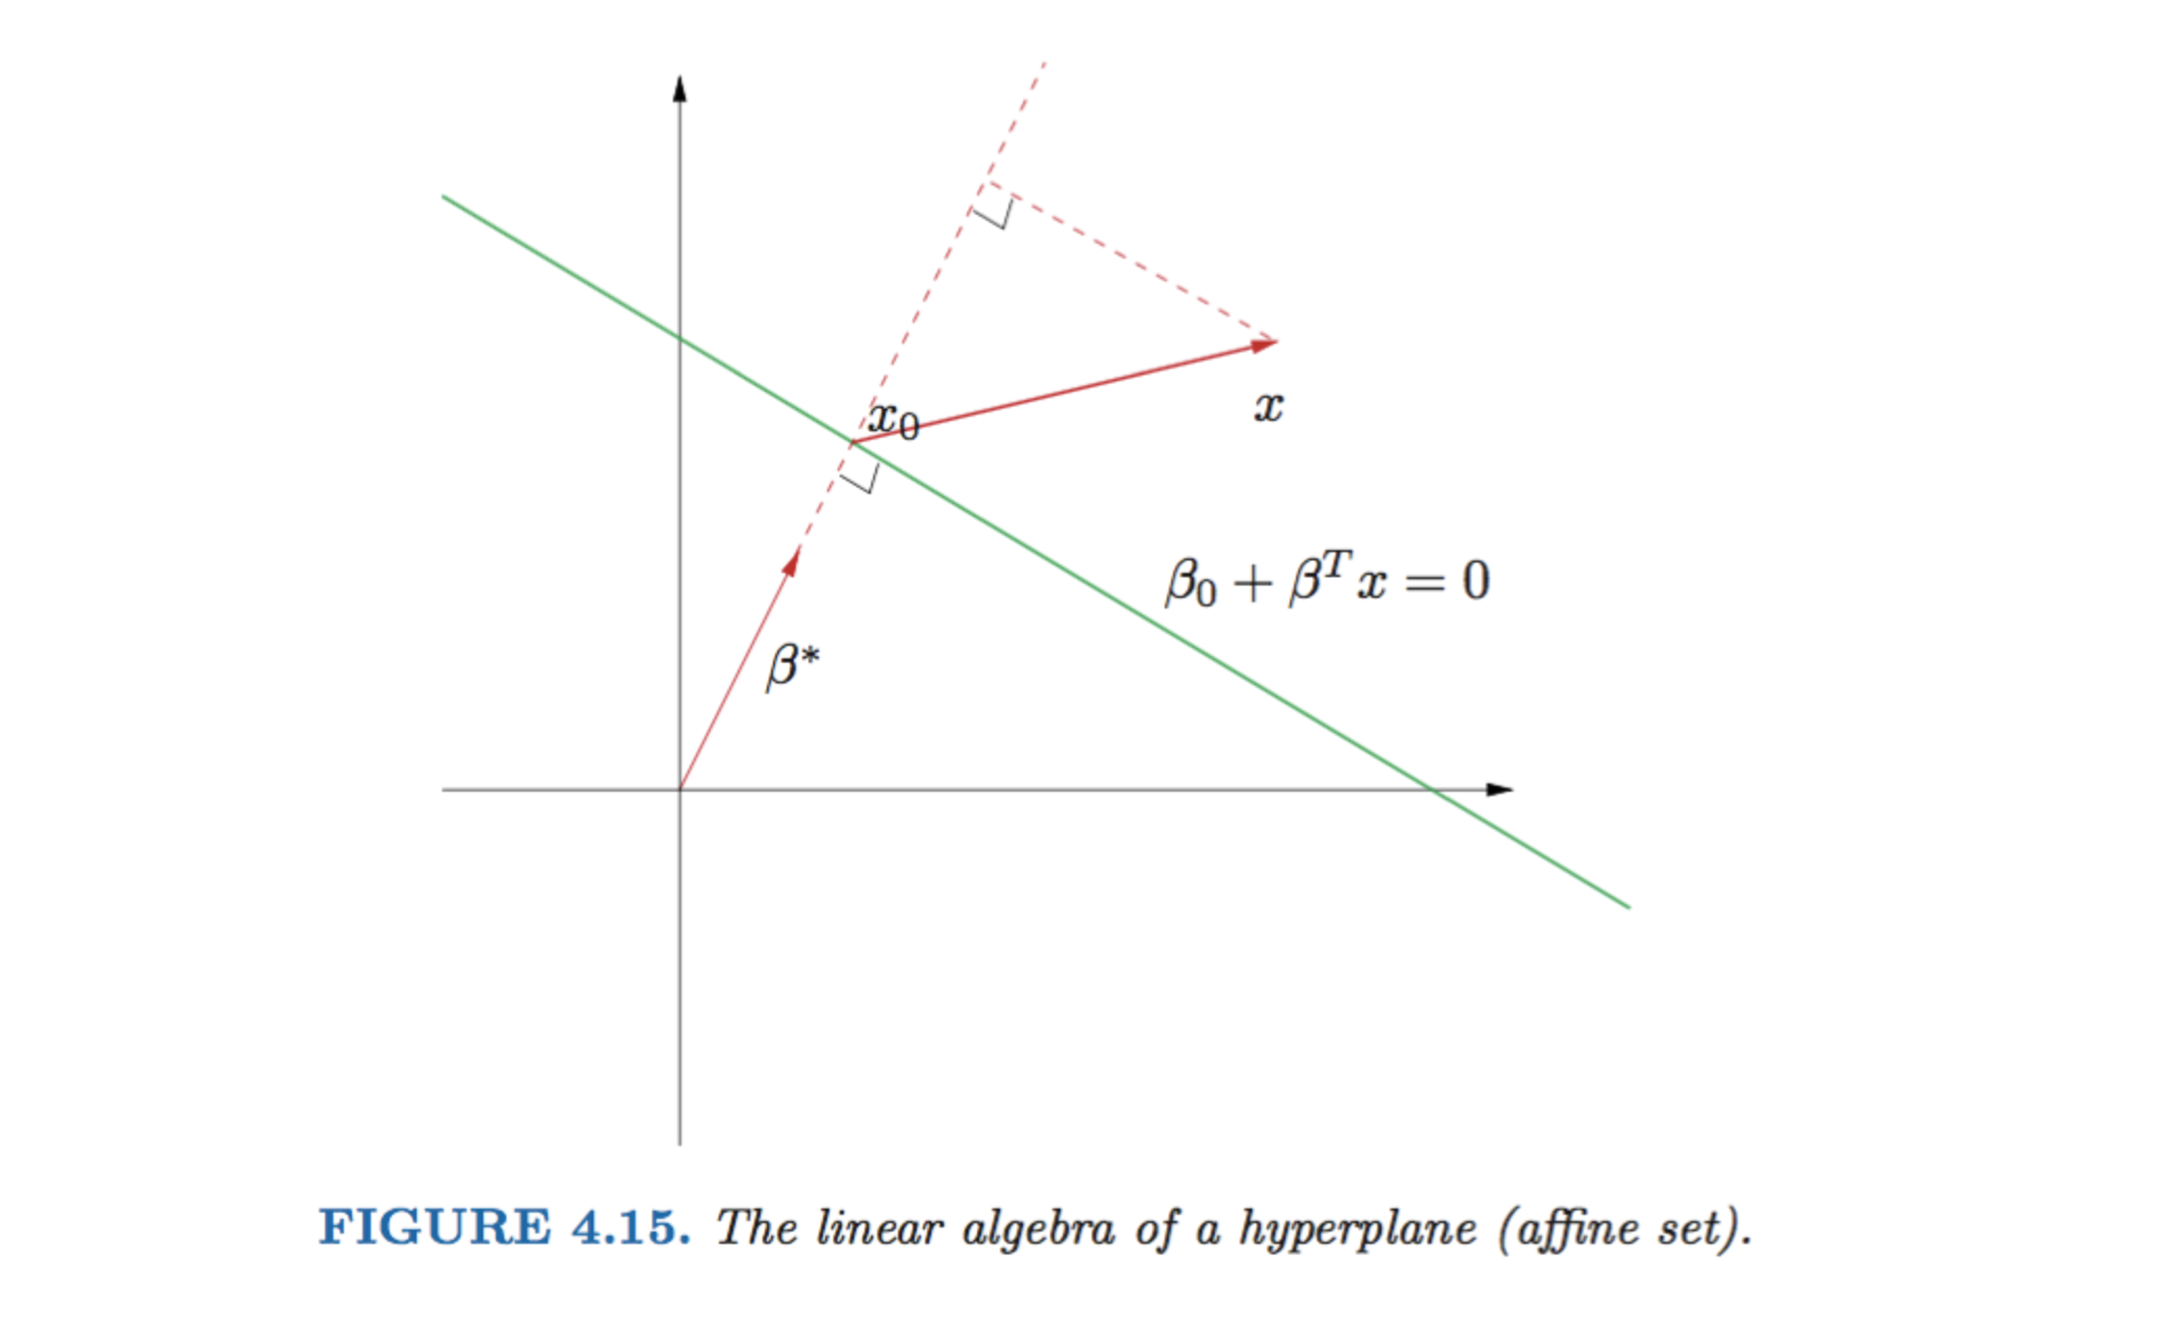
\includegraphics[height=0.7\textheight]{img/hyperplane.pdf}
\end{center}

\end{frame}

%%%%%%%%%%%%%%%%%%%%%%%%%%%%%%%%%%%%%%%%%%%%%%%%%%%
\begin{frame}[fragile] \frametitle{} \oldB \small

\textbf{\yblue{Linear Classification Models, cont.}}

Let's look at this using a small two dimensional example.

\end{frame}

%%%%%%%%%%%%%%%%%%%%%%%%%%%%%%%%%%%%%%%%%%%%%%%%%%
{
\usebackgroundtemplate{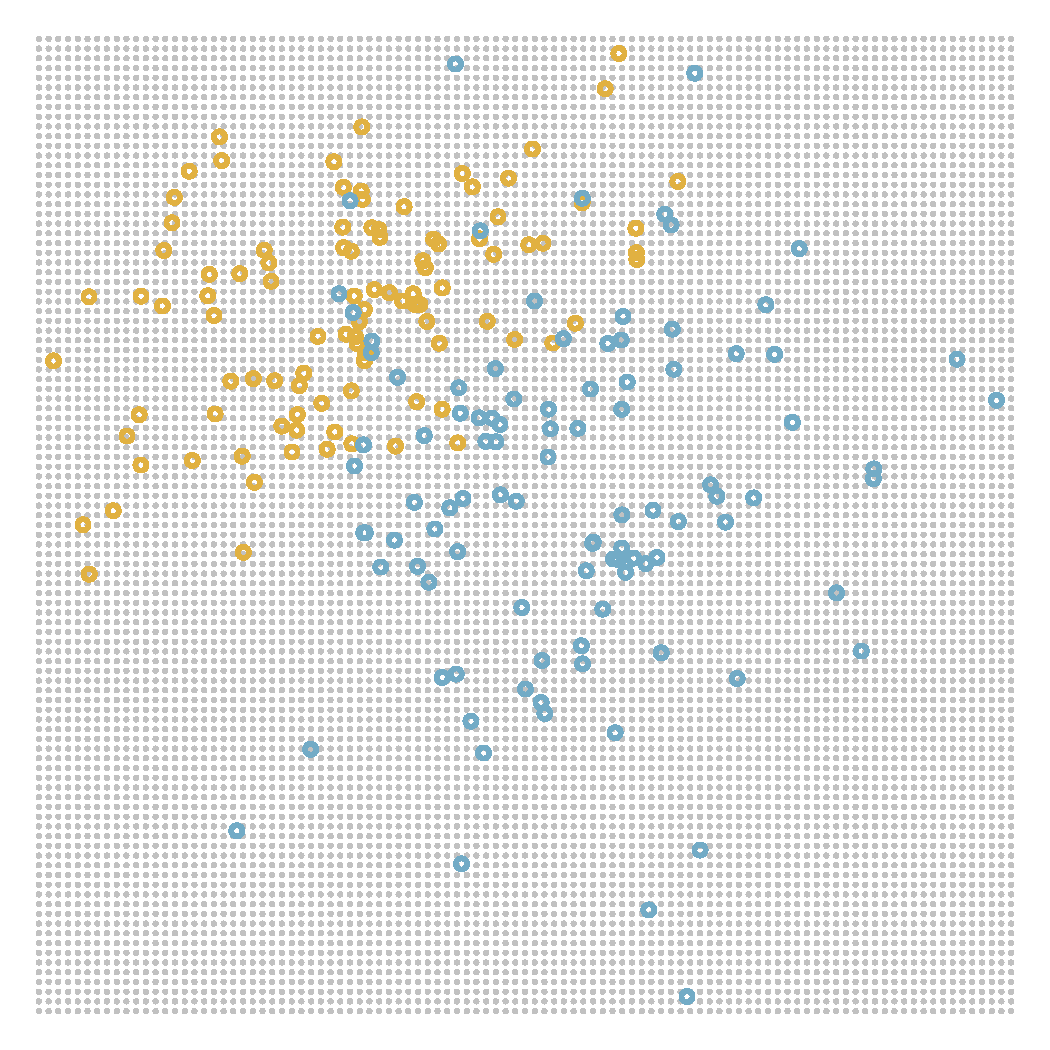
\includegraphics[height=\paperheight]{img/fig01.pdf}}
\begin{frame}[plain]
\end{frame}
}

%%%%%%%%%%%%%%%%%%%%%%%%%%%%%%%%%%%%%%%%%%%%%%%%%%
{
\usebackgroundtemplate{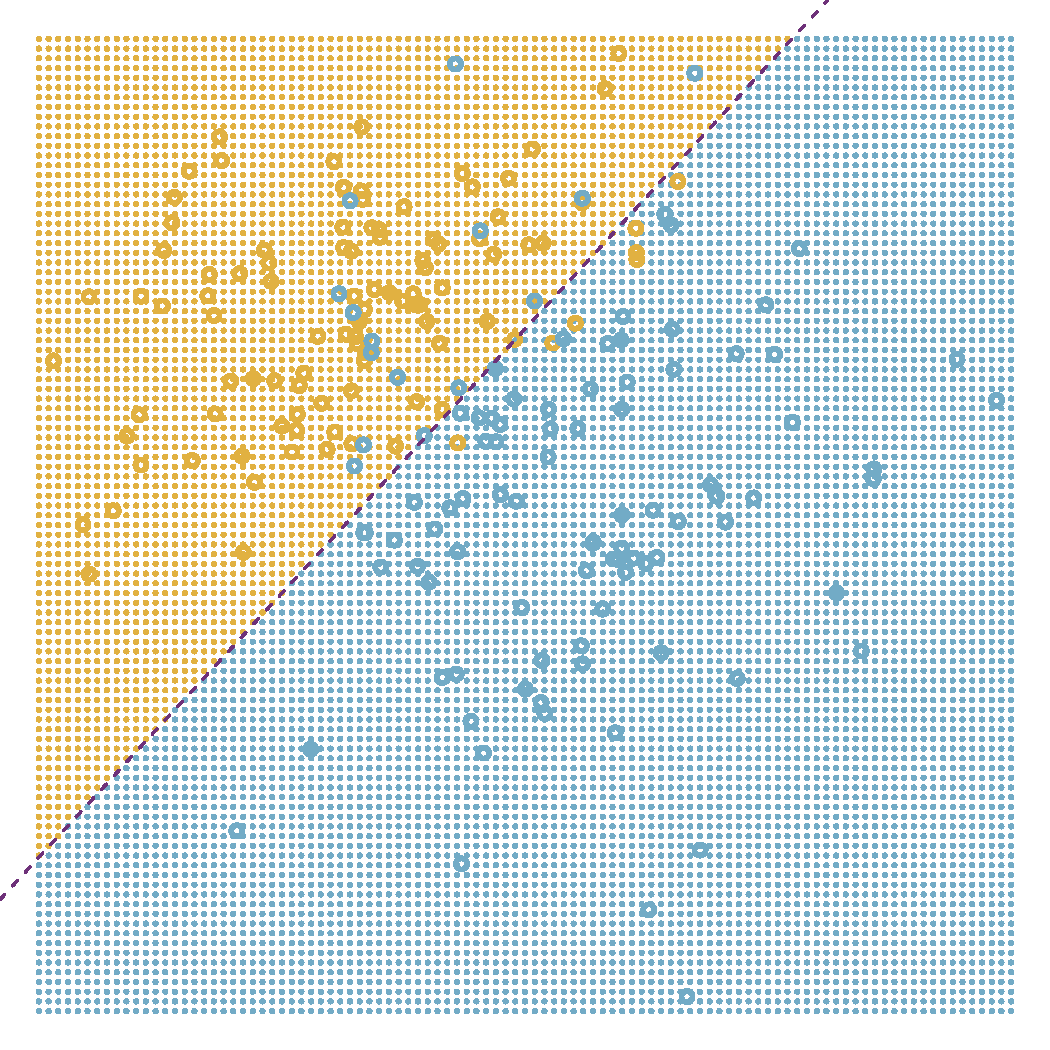
\includegraphics[height=\paperheight]{img/fig02.pdf}}
\begin{frame}[plain]
\end{frame}
}

%%%%%%%%%%%%%%%%%%%%%%%%%%%%%%%%%%%%%%%%%%%%%%%%%%%
\begin{frame}[fragile] \frametitle{} \oldB \small

\textbf{\yblue{Logistic regression}}

There is more than one way to estimate the best separating line that gives a
linear partition of the parameter space into two classes. One commonly used
example is \magenta{logistic regression}.

For this discussion, I'll re-parameterize the response variable $y$ to be
$0$ and $1$.

\end{frame}

%%%%%%%%%%%%%%%%%%%%%%%%%%%%%%%%%%%%%%%%%%%%%%%%%%%
\begin{frame}[fragile] \frametitle{} \oldB \small

\textbf{\yblue{Logistic regression, cont.}}

Consider a model where we assume that for each $y_i$ there exists an unknown
$p_i$ such that:
\begin{align}
\mathbb{P} \left[ y_i = 0 \right] &= 1 - p_i \\
\mathbb{P} \left[ y_i = 1 \right] &= p_i
\end{align}
In statistical terminology, we would say that $y_i$ is a random variable with
a Bernoulli distribution with parameter $p_i$.

\end{frame}

%%%%%%%%%%%%%%%%%%%%%%%%%%%%%%%%%%%%%%%%%%%%%%%%%%%
\begin{frame}[fragile] \frametitle{} \oldB \small

\textbf{\yblue{Logistic regression, cont.}}

Now, we want to somehow specify a relationship between a set of predictor
variables $x_i$ and the value $p_i$. A common selection is to use the logit
function:
\begin{align*}
p_i &= \frac{1}{1 + e^{-(x_i^t \beta + \beta_0)}}
\end{align*}
This has some deeper motivations if we look at the theory of exponential families
or describe the quantity in terms of the log-odds ratio.

For us, just notice that if $x_i \beta + \beta_0$ is zero, we get a $p_i$ of
$0.5$. When the linear quantity goes to positive infinity, the probabilities
go to $1$, and likewise when limiting to negative infinity, the probabilities go
to zero.

\end{frame}


%%%%%%%%%%%%%%%%%%%%%%%%%%%%%%%%%%%%%%%%%%%%%%%%%%%
\begin{frame}[fragile] \frametitle{} \oldB \small

\textbf{\yblue{Logistic regression, cont.}}

How do we use this formulation to actually predict the $\widehat{\beta}$ and
$\widehat{\beta}_0$? The standard approach is to use maximum likelihood estimation.
In short, we maximize the probability of observing the data $y_i$ conditioned on
the estimated parameters and the $x_i$'s.

\pause Computational this can be done by a modified form of iteratively re-weighted least
squares. Conceptually, we iteratively fit models that look like this:
\begin{align*}
\widehat{\gamma} &= (X^t W X)^{-1} X^t W y
\end{align*}
For some diagonal matrix of weights $W$. This is a second order method and converges quite
rapidly.

\end{frame}

%%%%%%%%%%%%%%%%%%%%%%%%%%%%%%%%%%%%%%%%%%%%%%%%%%%
\begin{frame}[fragile] \frametitle{} \oldB \small

\textbf{\yblue{Logistic regression, cont.}}

Notice that once again, we have a hyperplane defined by the set $x_i^t \beta + \beta_0$
that gives a linear separation between the two classes we wish to categorize.

How does this compare to the plane produced by linear regression?

\end{frame}

%%%%%%%%%%%%%%%%%%%%%%%%%%%%%%%%%%%%%%%%%%%%%%%%%%
{
\usebackgroundtemplate{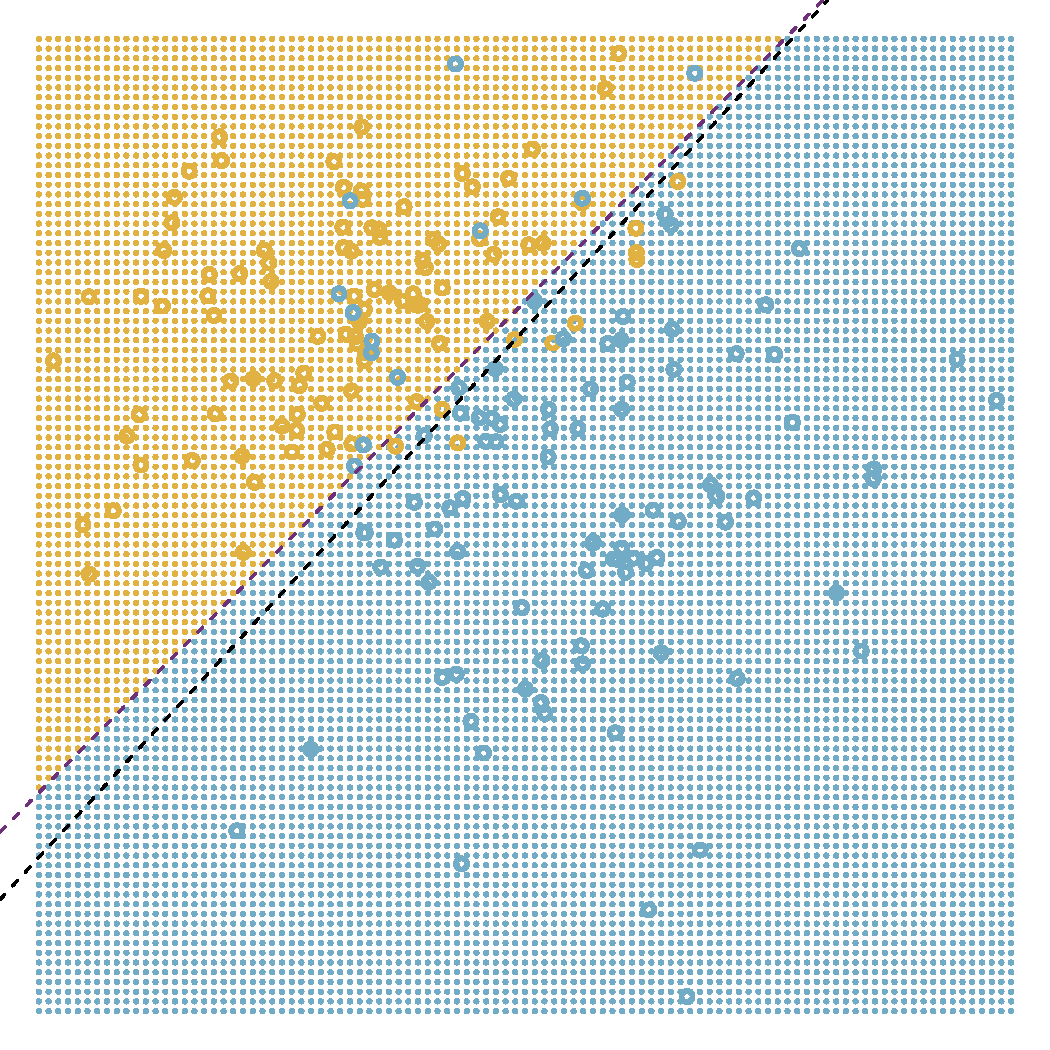
\includegraphics[height=\paperheight]{img/fig03.pdf}}
\begin{frame}[plain]
\end{frame}
}

%%%%%%%%%%%%%%%%%%%%%%%%%%%%%%%%%%%%%%%%%%%%%%%%%%%
\begin{frame}[fragile] \frametitle{} \oldB \small

\textbf{\yblue{Logistic regression, cont.}}

As with linear regression, we can do basis expansion to get non-linear classification
boundaries. So, for example, here we could treat $x_1^2$ and $x_1^3$ as the new third
and fourth dimensions of the predictor matrix. We learn a linear separating plane in
this higher dimensional space. However, when we project these predictions back down
into the original space, the effect is to give a non-linear boundary between the classes.

\end{frame}

%%%%%%%%%%%%%%%%%%%%%%%%%%%%%%%%%%%%%%%%%%%%%%%%%%
{
\usebackgroundtemplate{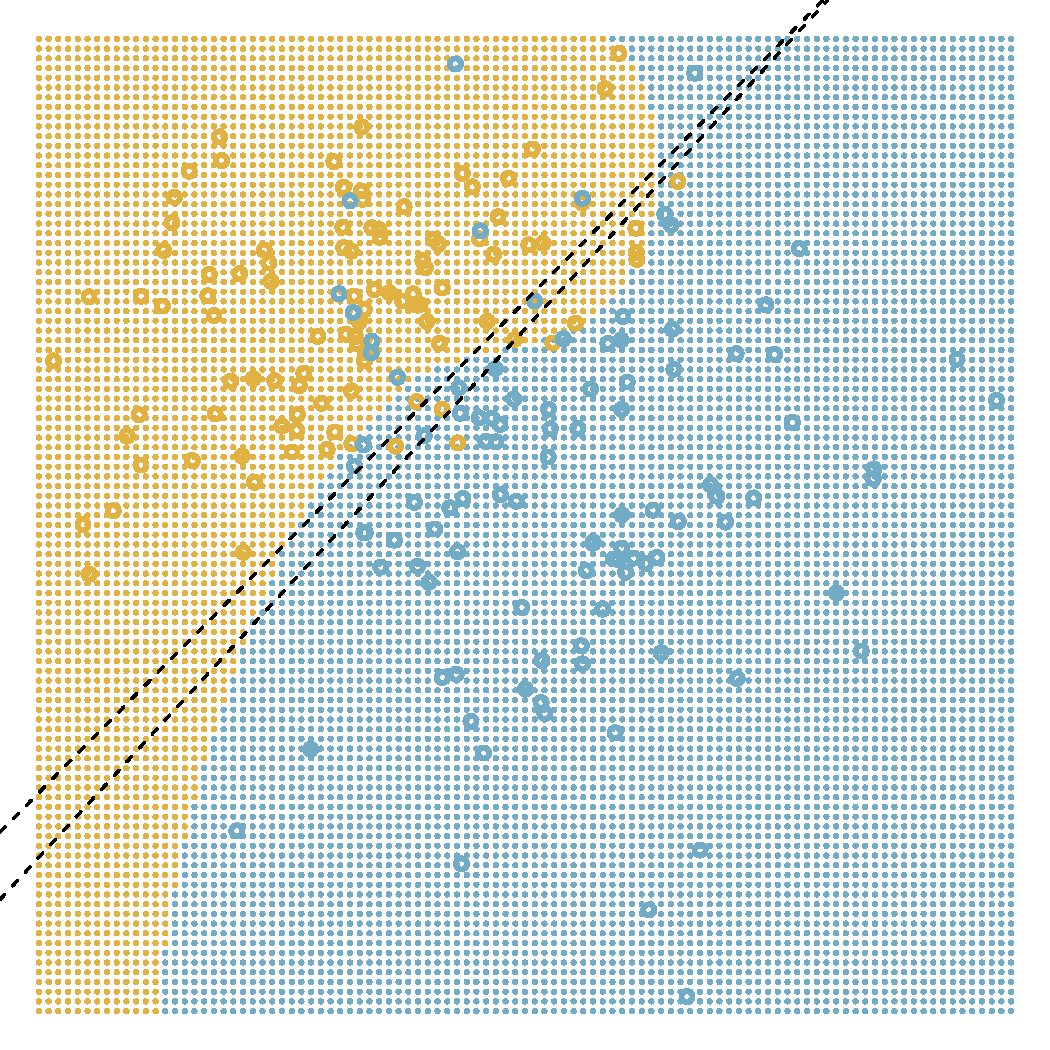
\includegraphics[height=\paperheight]{img/fig04.pdf}}
\begin{frame}[plain]
\end{frame}
}

%%%%%%%%%%%%%%%%%%%%%%%%%%%%%%%%%%%%%%%%%%%%%%%%%%%
\begin{frame}[fragile] \frametitle{} \oldB \small

\textbf{\yblue{Support vector machines}}

Support vector machines are powerful machine learning algorithms that also construct
separating planes for classification. They are conceptually fairly simple, but the
underlying mathematics for learning them from data can become a bit tricky.

\end{frame}

%%%%%%%%%%%%%%%%%%%%%%%%%%%%%%%%%%%%%%%%%%%%%%%%%%%
\begin{frame}[fragile] \frametitle{} \oldB \small

\textbf{\yblue{Support vector machines, cont.}}

The \magenta{linear}, \magenta{hard-margin} classification case can be described
quite succinctly: Pick two parallel hyperplanes that separate the two classes such
that the distance between the hyperplanes is maximal; the maximum-margin hyperplane
is the midpoint of these two separating planes.

\end{frame}

%%%%%%%%%%%%%%%%%%%%%%%%%%%%%%%%%%%%%%%%%%%%%%%%%%%
\begin{frame}[fragile] \frametitle{} \oldB \small

\begin{center}
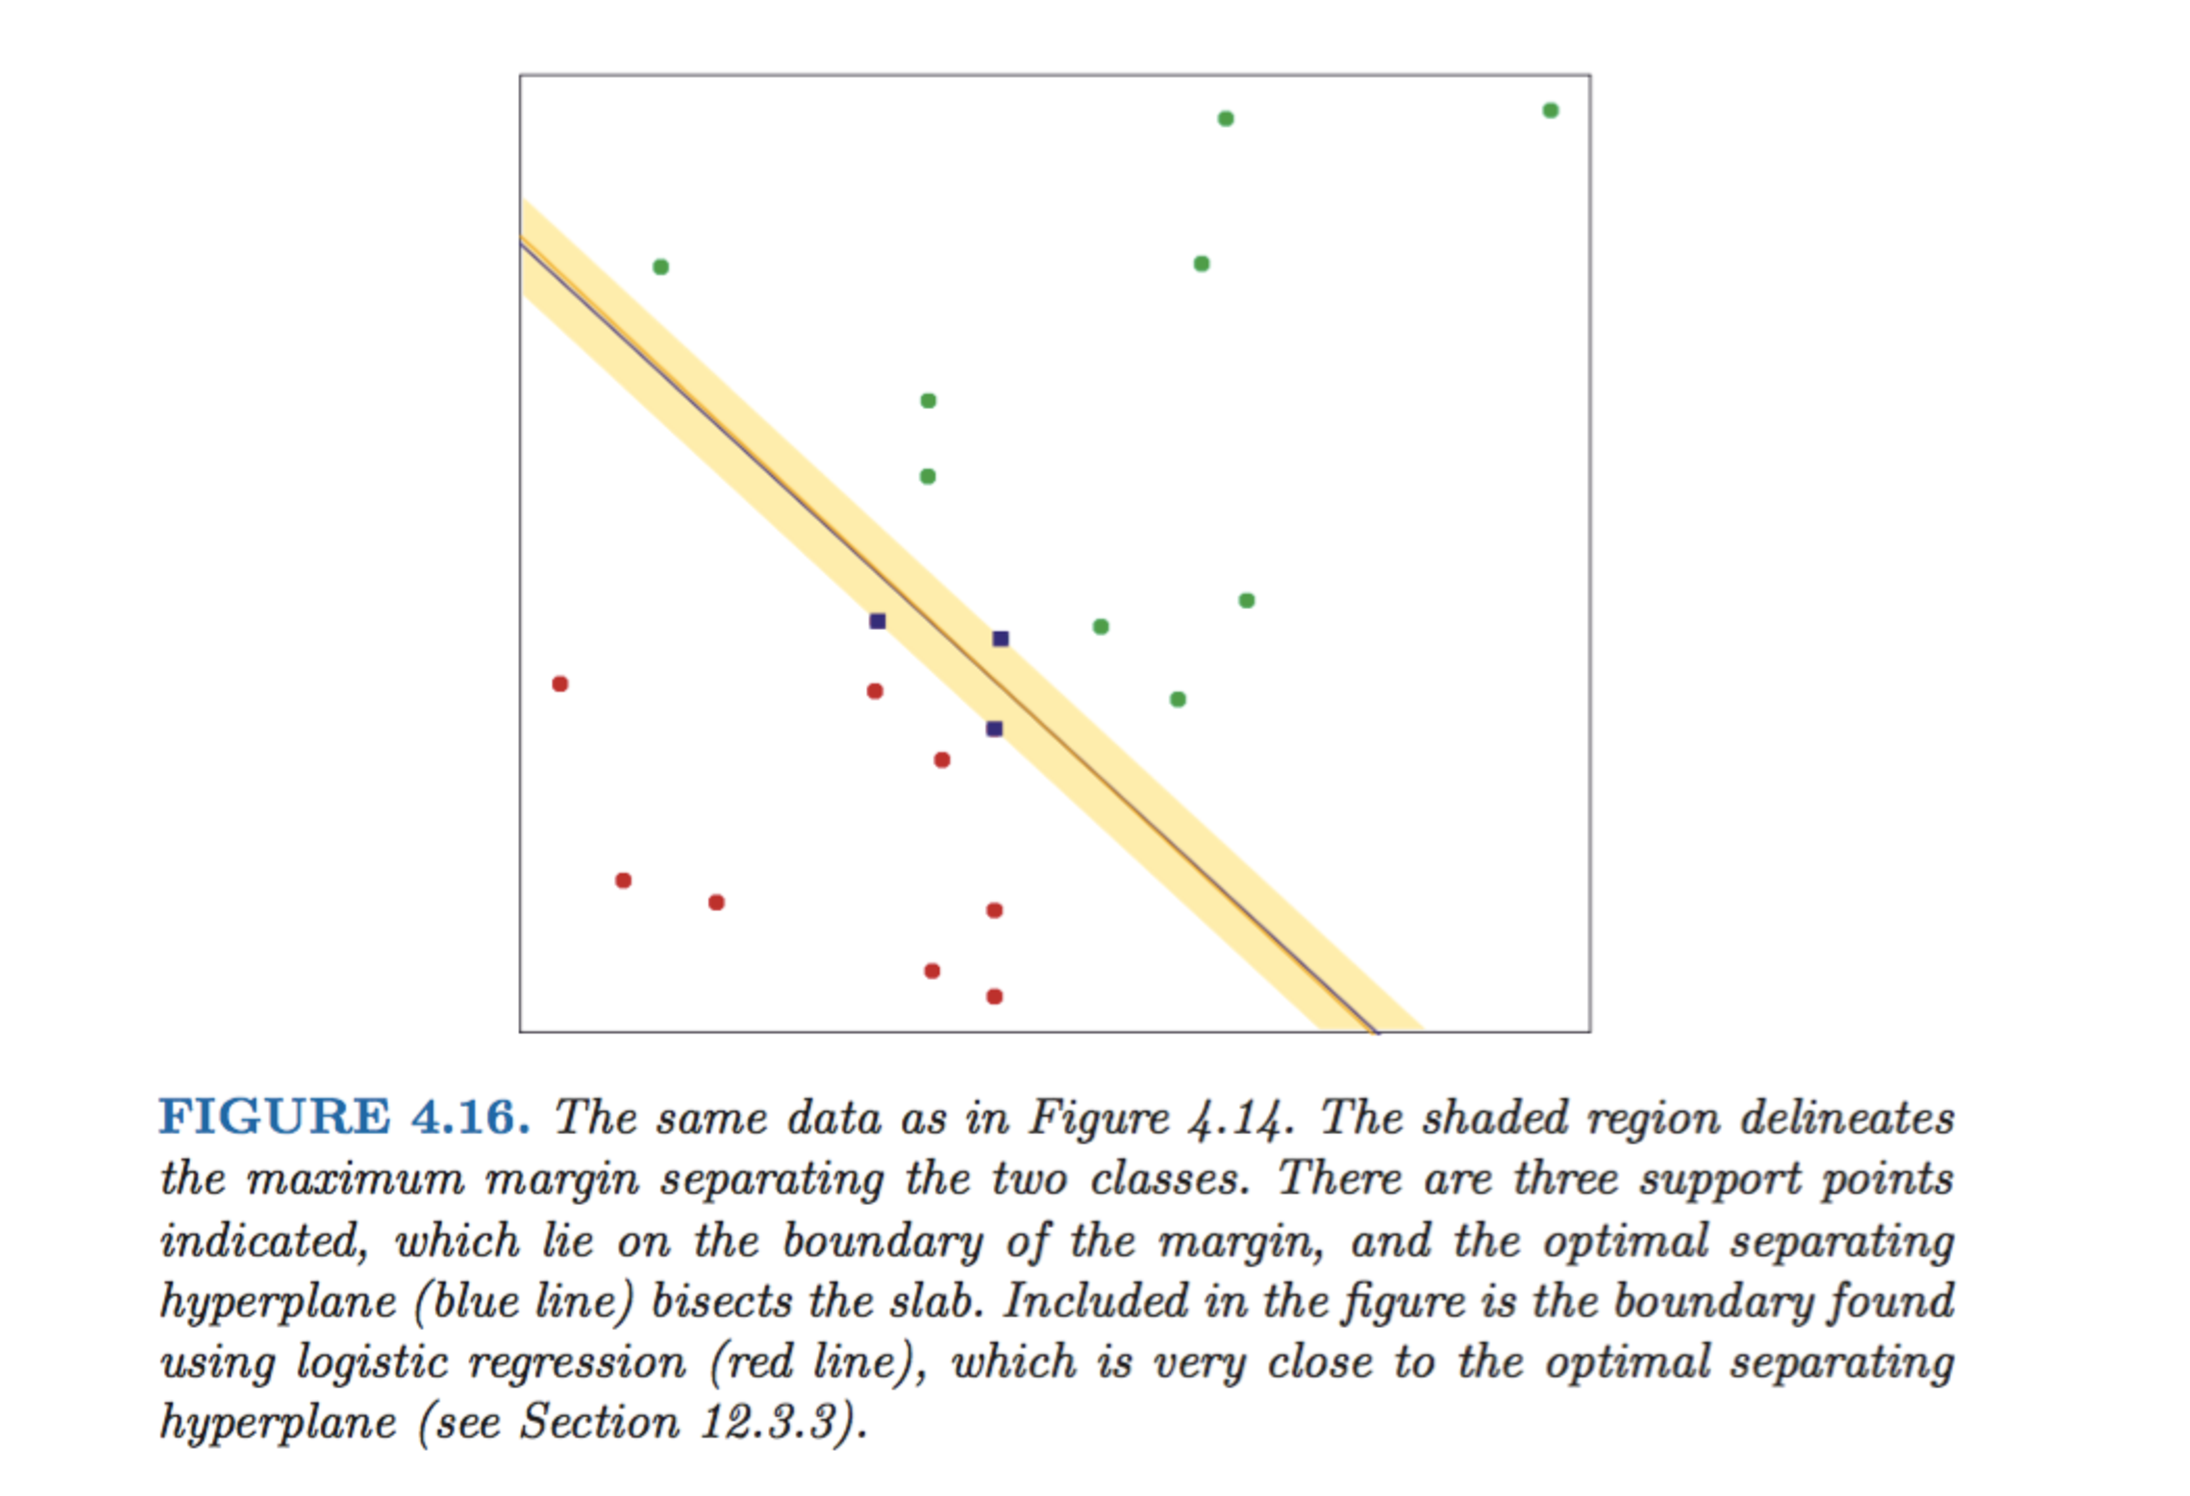
\includegraphics[height=0.7\textheight]{img/split.pdf}
\end{center}

\end{frame}

%%%%%%%%%%%%%%%%%%%%%%%%%%%%%%%%%%%%%%%%%%%%%%%%%%%
\begin{frame}[fragile] \frametitle{} \oldB \small

As we just saw, a hyperplane can be represented as the set:
\begin{align*}
\left\{ x \in \mathbb{R} \quad \text{s.t.} \quad \beta_0 + \beta^t x = 0 \right\}
\end{align*}
For a given $\beta_0$ and $\beta^t \in \mathbb{R}^p$. And the
`side' of the hyperplane that a point $x$ is on can be determined by:
\begin{align*}
\text{sign} \left( \beta_0 + \beta^t x \right)
\end{align*}

\end{frame}

%%%%%%%%%%%%%%%%%%%%%%%%%%%%%%%%%%%%%%%%%%%%%%%%%%%
\begin{frame}[fragile] \frametitle{} \oldB \small

Notice that we want $\beta_0 + \beta^t x_i$ to be positive if
$y_i$ is positive and negative if $y_i$ is negative. We can
then compactly write the necessary and sufficient condition for
a hyperplane correctly separating the input points:
\begin{align*}
y_i (x_i^t \beta + \beta_0) > 0, \quad i = 1, \ldots, n.
\end{align*}
\pause Assuming we have such a separating hyperplane, the minimal
value of the left hand side gives a measurement of the distance of
the closest point to the separating plane. In order to make this
distance consistent, we only consider for the moment $|| \beta ||_2 = 1$.

\end{frame}

%%%%%%%%%%%%%%%%%%%%%%%%%%%%%%%%%%%%%%%%%%%%%%%%%%%
\begin{frame}[fragile] \frametitle{} \oldB \small

Now, we have said that a support vector machine minimizes the margin
of a separating hyperplane. This can be written as:
\begin{align*}
\max_{|| \beta ||_2 = 1} \quad &  M \\
\text{s.t.} \quad & y_i (x_i^t \beta + \beta_0) > M, \quad i = 1, \ldots, n.
\end{align*}
The quantity $M$ is called the \magenta{margin}.

\end{frame}

%%%%%%%%%%%%%%%%%%%%%%%%%%%%%%%%%%%%%%%%%%%%%%%%%%%
\begin{frame}[fragile] \frametitle{} \oldB \small

It will be easier going forward to fix the value of $M$ to be $1$ and then
minimize the size of $\beta$:
\begin{align*}
\min \quad &  \frac{1}{2} || \beta ||_2^2 \\
\text{s.t.} \quad & y_i (x_i^t \beta + \beta_0) > 1, \quad i = 1, \ldots, n.
\end{align*}
Where the factor of $1/2$ and squared norm are added for later
notational convenience.

This defines a margin around the linear decision plane of width
$\frac{1}{|| \beta ||}$

\end{frame}

%%%%%%%%%%%%%%%%%%%%%%%%%%%%%%%%%%%%%%%%%%%%%%%%%%%
\begin{frame}[fragile] \frametitle{} \oldB \small

\begin{center}
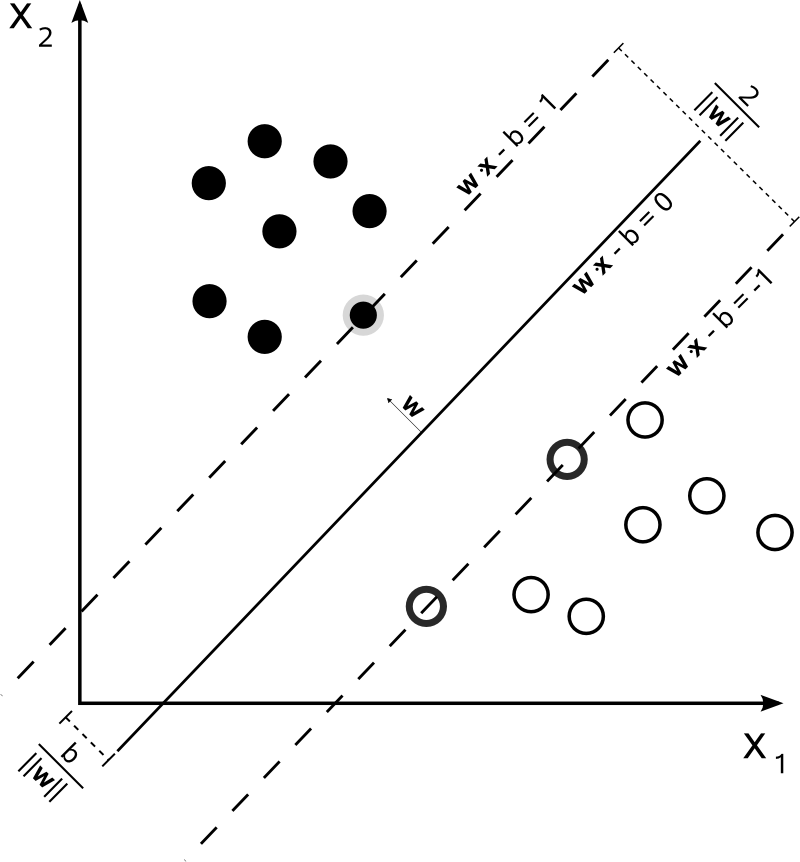
\includegraphics[height=0.7\textheight]{img/svmHardMargin.png}
\end{center}

\end{frame}

%%%%%%%%%%%%%%%%%%%%%%%%%%%%%%%%%%%%%%%%%%%%%%%%%%%
\begin{frame}[fragile] \frametitle{} \oldB \small

\textbf{\yblue{Soft margin and Cost Function}}

What happens, as in our original example, when there is not such separating
hyperplane? We introduce \magenta{slack variables} that produce a so-called
soft margin: the optimization algorithm has a certain amount of leeway in
allowing some points to be on the wrong side of the classification.

\end{frame}

%%%%%%%%%%%%%%%%%%%%%%%%%%%%%%%%%%%%%%%%%%%%%%%%%%%
\begin{frame}[fragile] \frametitle{} \oldB \small

Incorporating into our current specification, we add a $\xi_i$ for each
observation and rewrite our optimization problem as:
\begin{align*}
\min \quad &  \frac{1}{2} || \beta ||_2^2 \\
\text{s.t.} \quad & y_i (x_i^t \beta + \beta_0) > 1 - \xi_i, \quad i = 1, \ldots, n \\
\xi_i > 0, \, \sum_i \xi_i \leq \text{Constant}.
\end{align*}
So $\xi_i$ will be non-zero for mis-classified points, and the amount of
misclassification allowed is controlled by the constant in the model.

\end{frame}

%%%%%%%%%%%%%%%%%%%%%%%%%%%%%%%%%%%%%%%%%%%%%%%%%%%
\begin{frame}[fragile] \frametitle{} \oldB \small

\begin{center}
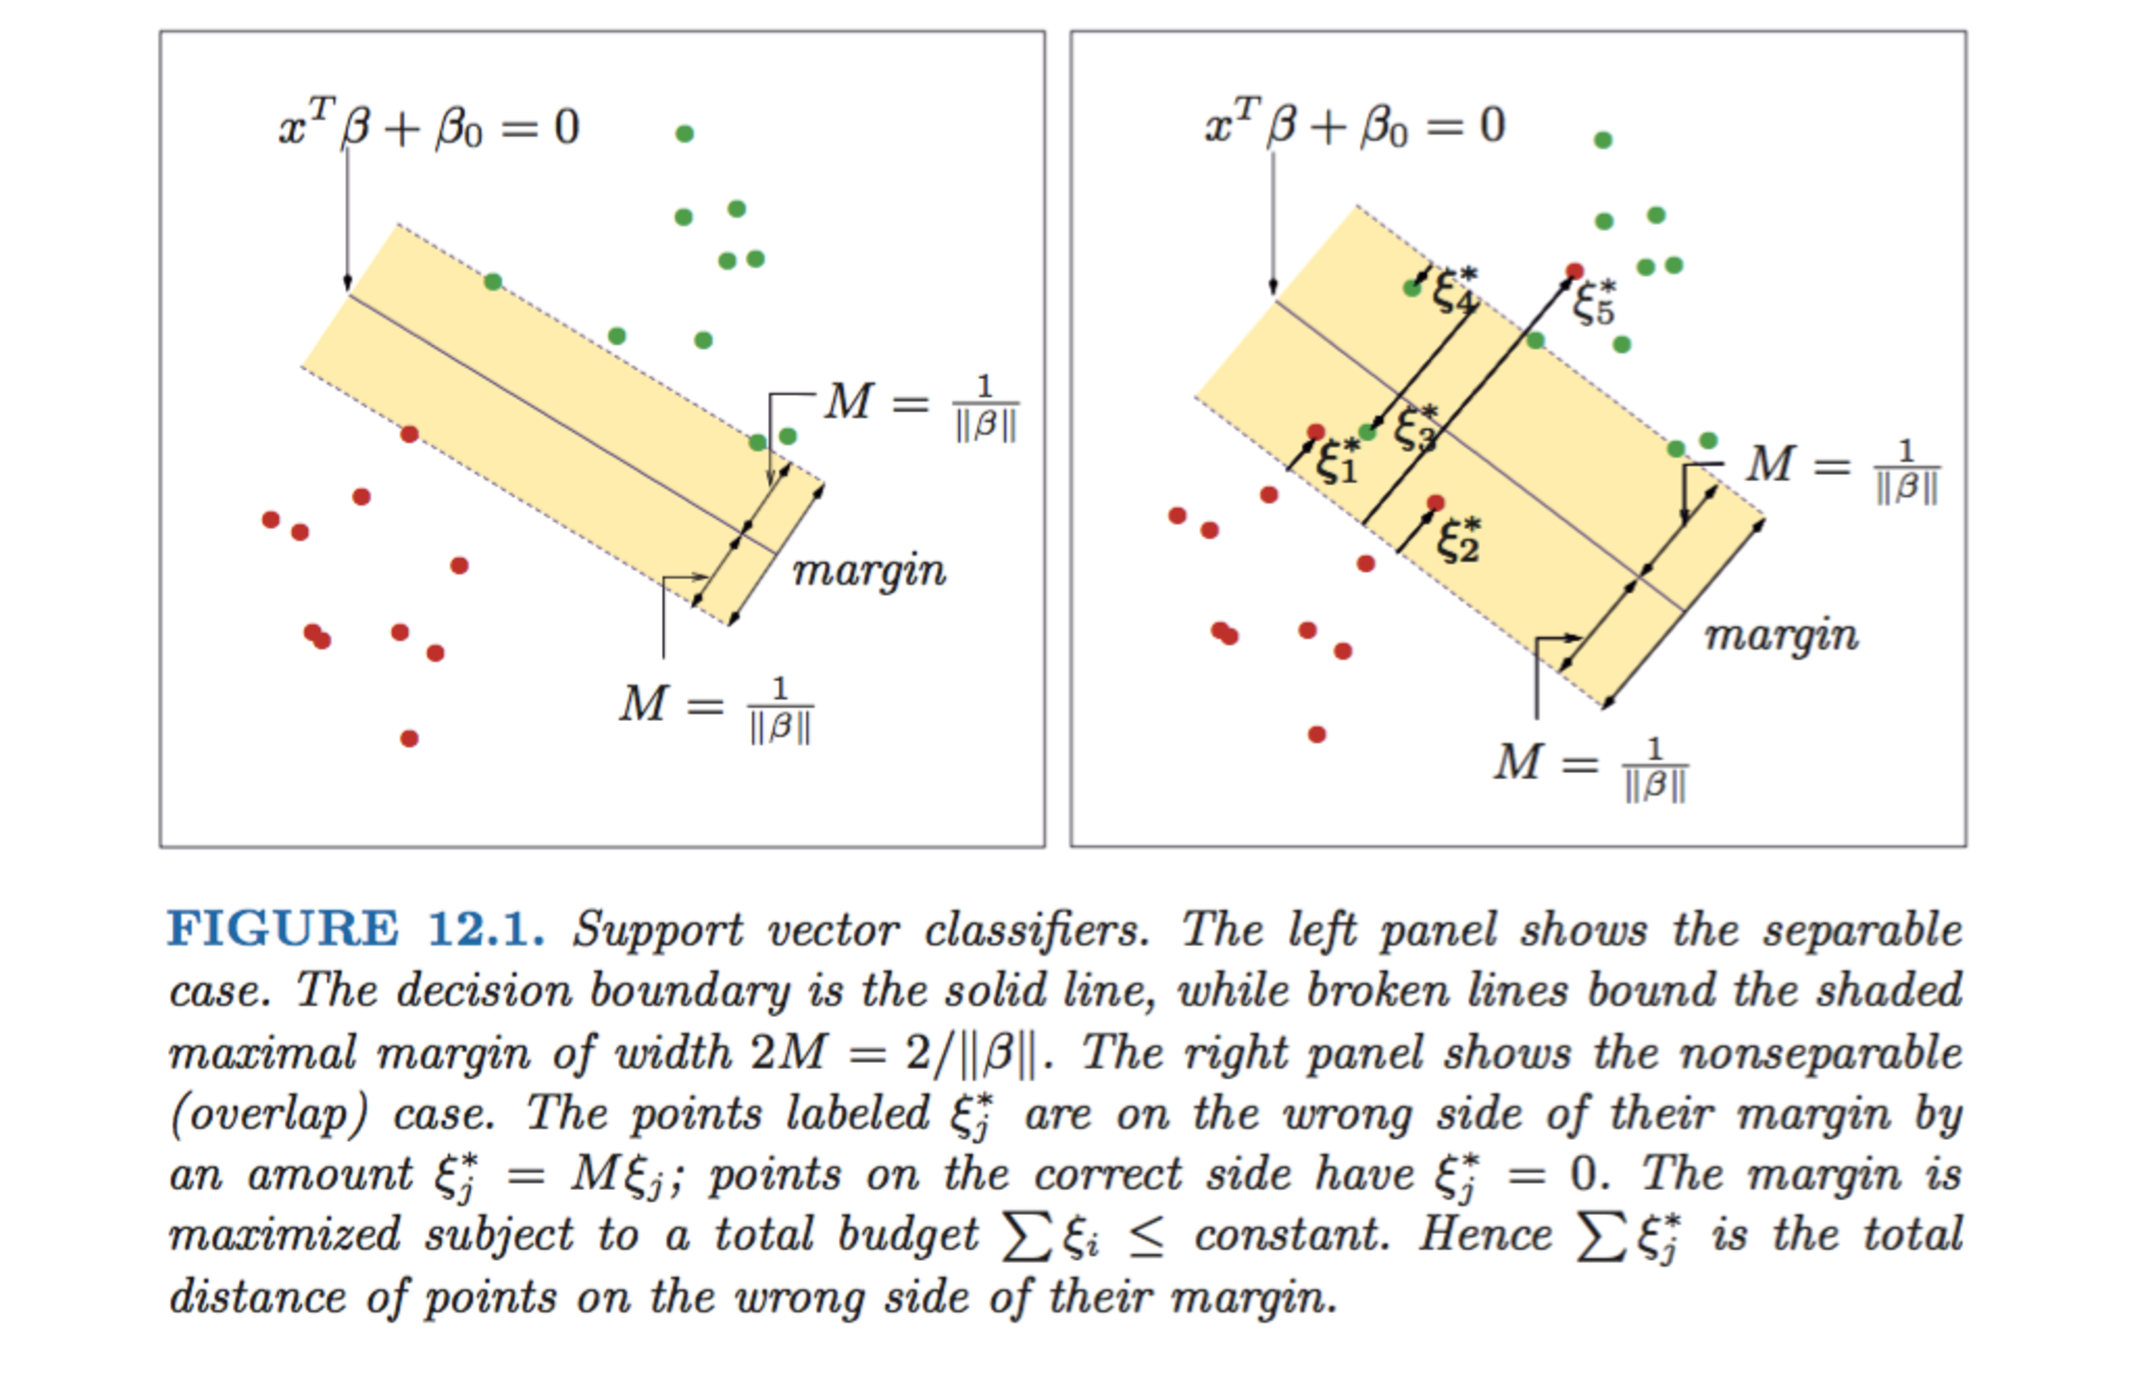
\includegraphics[height=0.7\textheight]{img/slack.pdf}
\end{center}

\end{frame}

%%%%%%%%%%%%%%%%%%%%%%%%%%%%%%%%%%%%%%%%%%%%%%%%%%%
\begin{frame}[fragile] \frametitle{} \oldB \small

\textbf{\yblue{Soft margin and Cost Function, cont.}}

So now, how does this boundary compare to the example we were working with
for linear and logistic regression?

\end{frame}

%%%%%%%%%%%%%%%%%%%%%%%%%%%%%%%%%%%%%%%%%%%%%%%%%%
{
\usebackgroundtemplate{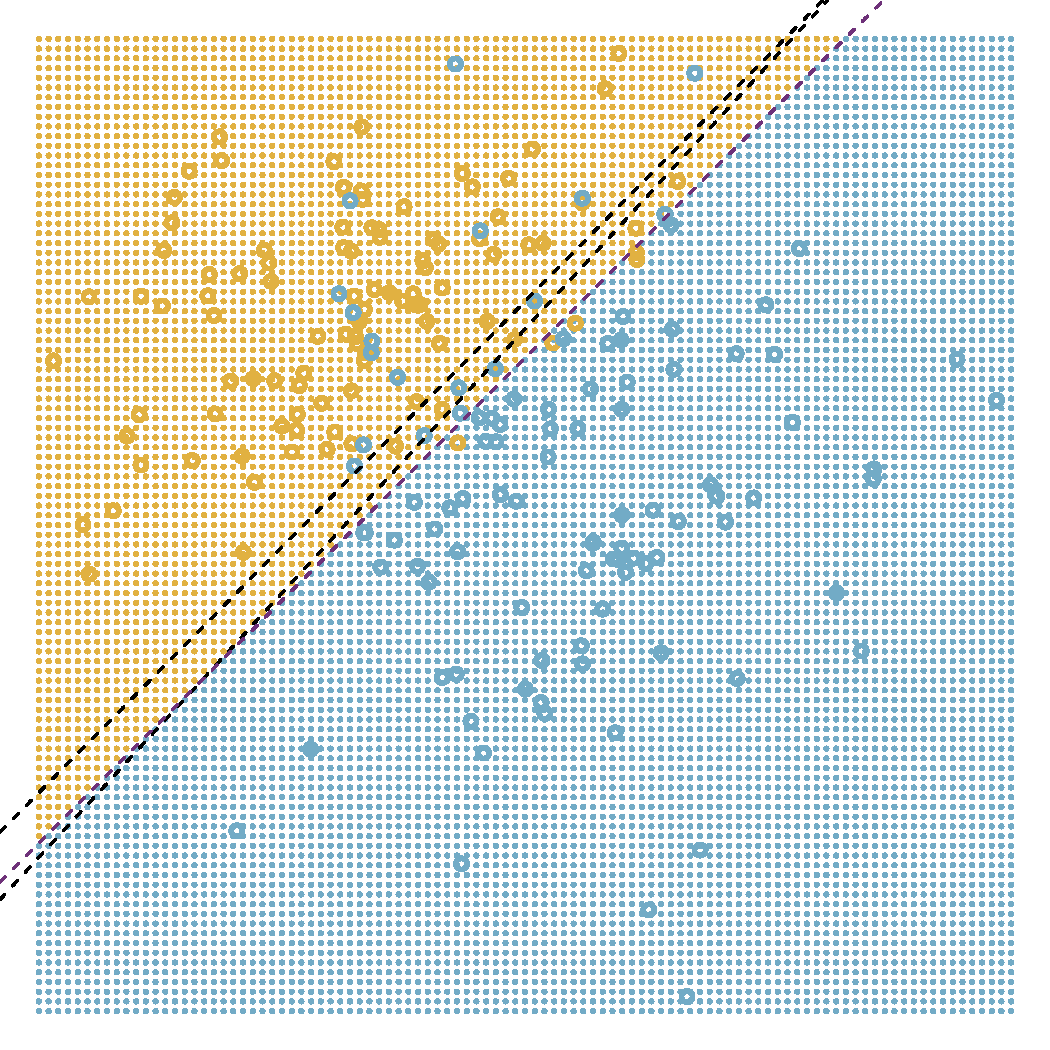
\includegraphics[height=\paperheight]{img/fig05.pdf}}
\begin{frame}[plain]
\end{frame}
}

%%%%%%%%%%%%%%%%%%%%%%%%%%%%%%%%%%%%%%%%%%%%%%%%%%%
\begin{frame}[fragile] \frametitle{} \oldB \small

\textbf{\yblue{Non-linear SVM}}

Much like linear and logistic regression, there is a way to do SVM in a higher
dimensional space via basis expansion in order to capture non-linear effects.

\end{frame}


%%%%%%%%%%%%%%%%%%%%%%%%%%%%%%%%%%%%%%%%%%%%%%%%%%
{
\usebackgroundtemplate{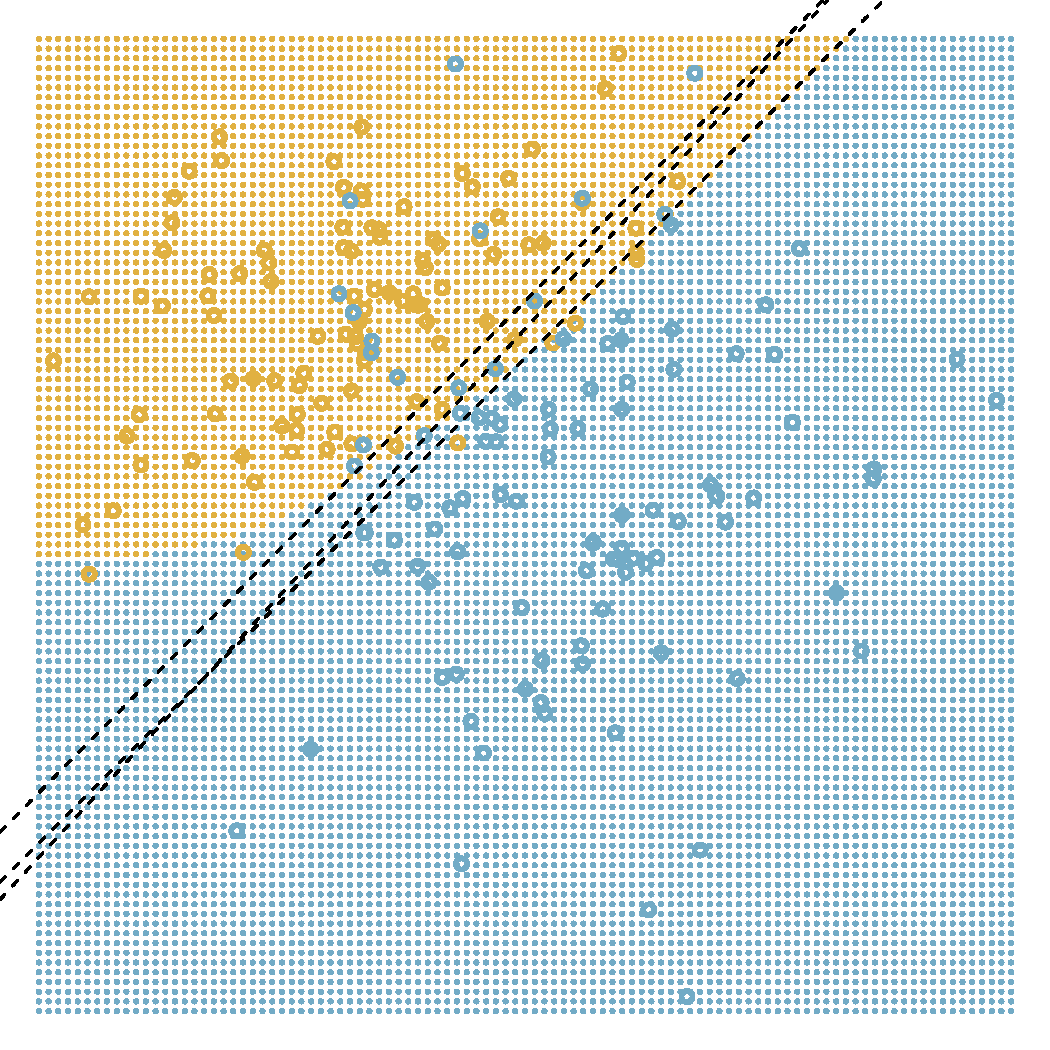
\includegraphics[height=\paperheight]{img/fig06.pdf}}
\begin{frame}[plain]
\end{frame}
}

%%%%%%%%%%%%%%%%%%%%%%%%%%%%%%%%%%%%%%%%%%%%%%%%%%%
\begin{frame}[fragile] \frametitle{} \oldB \small

\textbf{\yblue{Next for SVMs}}

So we have only scratched the surface of some of the interesting complexity of
support vector machines. Next time I'll delve into the actual computational
aspects of optimizing the SVM equations. This is actually quite important to
understand as it gives us more intuition for why they are so predictive in
higher dimensional spaces.

\end{frame}


\end{document}











